\documentclass{article}% {\twocolumn}
\usepackage{listings}
\usepackage{xcolor}
\usepackage{amsmath}
\usepackage{amssymb}
\usepackage{stmaryrd}
\usepackage{url}

\usepackage{graphicx}
\graphicspath{ {../../../assets/} }

\newcommand{\bR}{\mathbb{R}}
\newcommand{\lift}{\text{lift}}

\definecolor{codegreen}{rgb}{0,0.6,0}
\definecolor{codegray}{rgb}{0.5,0.5,0.5}
\definecolor{codepurple}{rgb}{0.58,0,0.82}
\definecolor{backcolour}{rgb}{0.95,0.95,0.92}

\lstdefinestyle{mystyle}{
    language=Python,
    backgroundcolor=\color{backcolour},   
    commentstyle=\color{codegreen},
    keywordstyle=\color{magenta},
    numberstyle=\tiny\color{codegray},
    stringstyle=\color{codepurple},
    basicstyle=\ttfamily\footnotesize,
    breakatwhitespace=false,         
    breaklines=true,                 
    captionpos=b,                    
    keepspaces=true,                 
    numbers=left,                    
    numbersep=5pt,                  
    showspaces=false,                
    showstringspaces=false,
    showtabs=false,                  
    tabsize=2
}

\lstset{style=mystyle}

\begin{document}


\title{Lifting E-Graphs: A Function Isn't a Constant}

\author{Philip Zucker}

\maketitle
\begin{abstract}
Variables are quite subtle and easy to get wrong. An approach to support a notion of rigid $\alpha$ canonical variables in e-graphs inspired by slotted e-graphs \cite{slotted} and Co-de Bruijn syntax \cite{McBride_2018} is described. The e-graph can be seen as having a baked-in notion of functional lifting combinator implemented by fattening integer identifiers with thinning bitvectors, lift pulling smart constructors, and a special thinning aware union find variation.
\end{abstract}

\section{Introduction}
E-graphs \cite{egg} are a data structure that compactly store ground terms and equalities between them.

 E-graphs are supposed to be useful for program optimization, and program expressions usually have unknowns such as  $x * 2 / 2$. From the outset, E-graphs have had variables in them.

There are a number of issues with explicit names like $x$ in the e-graph setting

\begin{enumerate}
\item Generative processes like equality saturation can run off the rails if fresh names are created via a gensym for example in the rewrite rule $P \rightarrow \forall x, P$ or $e \rightarrow \frac{1}{N} \sum_{i=0}^{N-1} e$
\item The bidirectional nature of equality in an e-graph can cause scope hygiene concerns. The equality $x * 0 = 0$ can cause $x$ to appear in a context which does not have $x$ bound if named variables are treated naively, for example $\text{lam}(y, 0) = \text{lam}(y,x * 0)$
\item Named variables cause missed sharing. $\texttt{f(g(h(x)))}$ shares no storage with $\texttt{f(g(h(y)))}$. The amount of missed storage opportunity gets worse the deeper and bigger the term. Note that these two terms \emph{aren't equal}, but there is a missed \emph{relationship} that can be used for reasoning and compaction.
\item Depending on your intended semantics, expressions like $\sin(x)$ may ambiguously refer to multiple semantic entities. In other words, there may be \emph{too much} sharing. 
\end{enumerate}

\subsection{Which $\sin$ is $\sin(x)$?}

$\sin(x)$ from an ordinary perspective is fine. We've lived with the notation for hundreds of years. It works. We know what it means when we see it.

From another perspective it is horribly vague and possibly collapsing distinct entities. We are somehow referring vaguely to the function $\sin$, but are we specifically referring to $x \mapsto \sin(x) : R^1 \to R$ or to $x,y \mapsto \sin(x) : R^2 \to R$?

\begin{figure}[htbp]
\centering
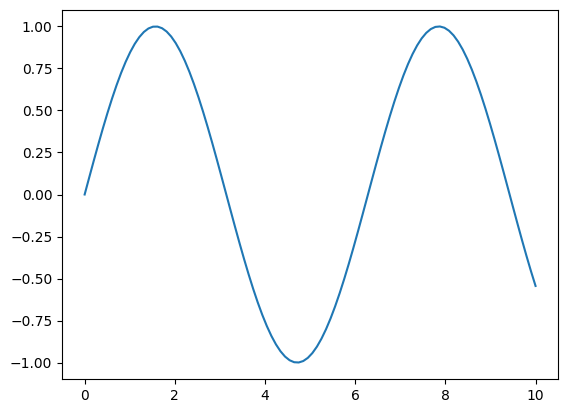
\includegraphics[width=0.5\linewidth]{2026-04-18-thin_egraph_files/2026-04-18-thin_egraph_2_1.png}
\caption{$x \mapsto \sin(x) : R \to R$}
\label{fig:sin-r-to-r}
\end{figure}


\begin{figure}[htbp]
\centering
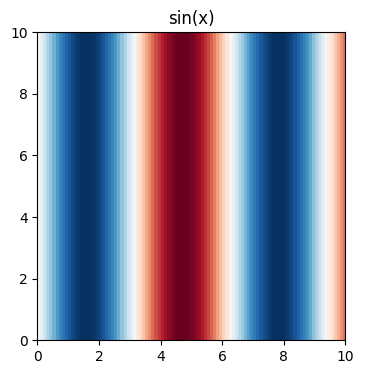
\includegraphics[width=0.5\linewidth]{2026-04-18-thin_egraph_files/2026-04-18-thin_egraph_6_crop.png}
\caption{$x,y \mapsto \sin(x) : R^2 \to R$}
\label{fig:sin-r2-to-r}
\end{figure}

These are different things. In fact, they can't even be compared for equality due to type mismatch. The two plots are completely different images. Yet, the notation that suppresses the context $x,y \mapsto \_$ or leaves it implicit conflates these two distinct things. It is at least worrying that perhaps in some subtle way this conflation is asserting $\bR^2 = \bR^1$ and from thence unsoundness ensues.

While it is not the case for every conception of the word "context" or the word "term", from this observation comes a design philosophy:

\textbf{The context $x,y \mapsto \_$ is not \emph{where} a term is, it is part of \emph{what} a term is}

\section{Naive Well-Dimensioned Nameless Representation}

It is helpful to find a way to talk about this less familiar $x,y \mapsto \_$  notation in the more standard framework of first order terms.

If there is an ambiguity about dimension, an simple approach to break this ambiguity is to add a $d$ dimension subscript everywhere.

We can make a different copy of every function symbol for every dimension/context we might be working in and we can refer to variables by (dimension,index) pairs $x_{di}$ rather than by names. For example $x \mapsto x$ becomes $\text{var}_{10}$ (the zeroth variable in context of size 1) and $x,y \mapsto y$ becomes $\text{var}_{21}$ (the first variable in context of size 2).

Likewise, we could also disambiguate all the $\sin$ into different versions $\sin_d$ depending on the type of its argument. If $\text{var}_{21}$ has type $\bR^2 \rightarrow \bR$ then if $\sin$ is going to accept it, it needs to take in arguments of that type. We have $\sin_0 : (\bR^0 \rightarrow \bR) \rightarrow (\bR^0 \rightarrow \bR)$, $\sin_1 : (\bR^1 \rightarrow \bR) \rightarrow (\bR^1 \rightarrow \bR)$,  $\sin_2 : (\bR^2 \rightarrow \bR) \rightarrow (\bR^2 \rightarrow \bR)$ and so on.

There is a pointwise compositional semantics of these combinators. 

\[
\begin{aligned}
\llbracket 42_d \rrbracket &= v_0, v_1, \ldots, v_{d-1} \mapsto 42 \\
\llbracket \operatorname{var}_{di} \rrbracket &= v_0, v_1, \ldots, v_{d-1} \mapsto v_i \\
\llbracket \sin_d(t) \rrbracket &= v_0, v_1, \ldots, v_{d-1} \mapsto \sin(\llbracket t \rrbracket(v_0, v_1, \ldots, v_{d-1})) \\
\llbracket t +_d s \rrbracket &= v_0, v_1, \ldots, v_{d-1} \mapsto \llbracket t \rrbracket(v_0, v_1, \ldots, v_{d-1}) + \llbracket s \rrbracket(v_0, v_1, \ldots, v_{d-1}) \\
&\text{and so on...}
\end{aligned}
\]

Semantically, $\operatorname{var}_{di}$ is a \emph{projection} of type $\mathbb{R}^d \rightarrow \mathbb{R}$. $\sin_d$ is a \emph{higher order function} of type $(\mathbb{R}^d \rightarrow \mathbb{R}) \rightarrow (\mathbb{R}^d \rightarrow \mathbb{R})$. It can also be viewed as the partial application of the composition function $\sin_d \sim \sin \circ (-)$.

Because we are being nameless by referring to variables by integers, $x \mapsto f(g(h(x)))$ becomes syntactically the same as $y \mapsto f(g(h(y)))$ since both become $f_1(g_1(h_1(\text{var}_{10})))$. So sharing in the e-graph using this representation has become better in that sense.

On the other hand, $\sin_1(\text{var}_{10}) : \mathbb{R}^1 \rightarrow \mathbb{R}$ and $\sin_2(\text{var}_{20}) : \mathbb{R}^2 \rightarrow \mathbb{R}$ now share no storage. This is fine from the perspective that they are not \emph{equal} (such a question does not even type check), but is disappointing from the perspective they are clearly \emph{related}.

\section{Lifting Functions for Increased Sharing}
Lifting is a functional combinator that drops some arguments and passes others along while maintaining their ordering. 

One way that $\sin_1(\text{var}_{10}) : \mathbb{R}^1 \rightarrow \mathbb{R}$ and $\sin_2(\text{var}_{20}) : \mathbb{R}^2 \rightarrow \mathbb{R}$ are related is by this operation of $\text{lift}_t : (\mathbb{R}^{\text{popcnt}(t)} \rightarrow \mathbb{R})\rightarrow (\mathbb{R}^{\text{len(t)}} \rightarrow \mathbb{R})$. For example $\text{lift}_{110} : (\mathbb{R}^{2} \rightarrow \mathbb{R})\rightarrow (\mathbb{R}^3 \rightarrow \mathbb{R})$  keeps arg 0, keeps arg 1, and drops arg 2.

It can be written as a simple Python combinator 

\begin{lstlisting}
def lift(thin : Thin):
    return lambda f: lambda *args: f(*act(thin, args))
\end{lstlisting}

Using this concept, we can make the differently dimensioned $\sin$ expressions share subterms and hence achieve shared memory storage.

$$\sin_1(\text{var}_{10}) := \sin(\text{var})$$

$$\sin_2(\text{var}_{20}) := \text{lift}_{10}(\sin(\text{var}))$$

\begin{figure}[htbp]
\centering
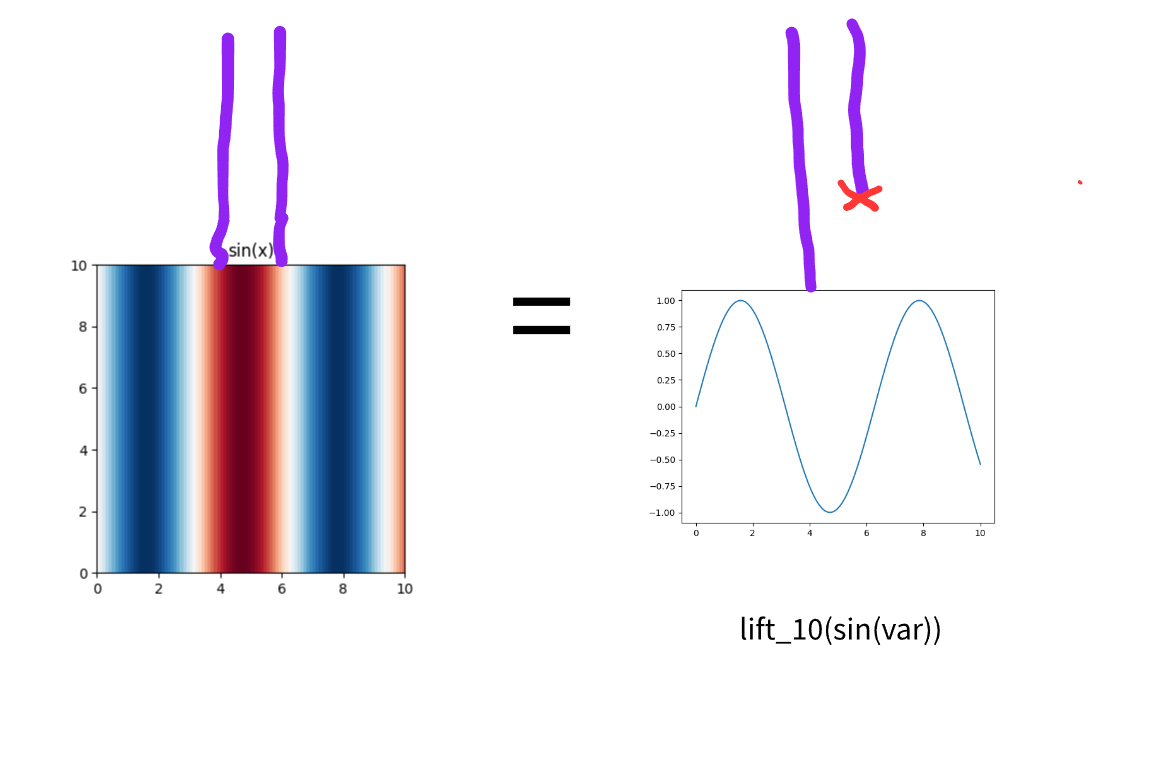
\includegraphics[width=0.5\linewidth]{thin_sin_sin.png}
\caption{A lifted sine expression}
\label{fig:thin-sin-sin}
\end{figure}

%![width:600](https://www.philipzucker.com/assets/thin_sin_sin.png)

The lifting is parametrized by a thinning\cite{McBride_2018}\cite{zucker2026thinningssub} bitvector $t$ with a $1$ for arguments to keep and $0$ for arguments to drop. One \emph{lifts} a function by \emph{thinning} its arguments list.

Thinnings can be thought of in a number of ways. They are strictly monotonic maps between totally ordered finite sets. They can also be seen as a recipe to extract subsequences.

They are similar mathematical objects to permutations, albeit more minimalist in data requirements and implementations. They can be seen as a compaction of multiple de Bruijn shifts in a manner similar to how a permutation dictionary is a compaction of many swaps \cite{zucker2026thinningssub}. When a de Bruijn shift occurs while pushing an expression inside of new binders, a gap is created between the indices referring to variables inside the expression and the indices referring to variables at the expression's original context. When one creates these gaps multiple times, one has created something akin to a thinning.

Thinnings have a notion of composition and identity. This makes them a category. They are relatives of the simplex category.


% If you gave me an object $\texttt{f1(g1(h1(x10)))} : R \to R$ I could produce the object $\texttt{f2(g2(h2(x20)))} : R^2 \to R$ by merely throwing away the second argument and propagating the first argument. As a python function, this lifting combinator would be written as  $\texttt{lambda f: lambda x,y: f(x)}$. This is a lifting operation, and lifting operations have a tractable algebra associated with them. \url{https://www.philipzucker.com/thin1/}

\begin{figure}[htbp]
\centering
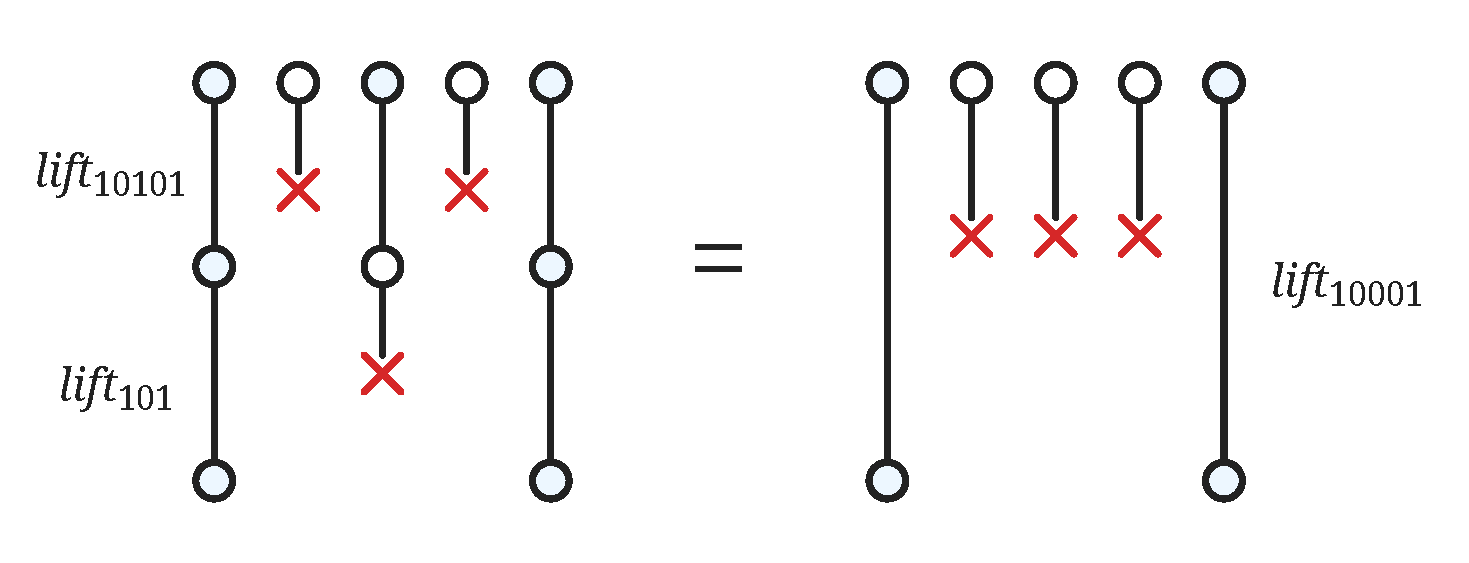
\includegraphics[width=0.5\linewidth]{thinning/simple-thinning.pdf}
\caption{Composition of thinnings}
\label{fig:compose-thinnings}
\end{figure}

\begin{lstlisting}
type Thin = list[bool]
def dom(f : Thin) -> int:
    return len(f)
def cod(f : Thin) -> int:
    return sum(f)
def id(n : int) -> Thin:
    return [True]*n
def comp(f : Thin, g : Thin) -> Thin:
    assert cod(f) == dom(g)
    i = 0 
    result = []
    for a in f:
        if a:
            result.append(g[i])
            i += 1
        else:
            result.append(False)
    assert i == len(g)
    return result
\end{lstlisting}

%Instead of ever storing $\texttt{f2(g2(h2(x20)))} : R^2 \to R$, I could instead store $\texttt{lift\_10(f1(g1(h1(x10))))} : R^2 \to R$. The subscript on $\lift$ is a bitvector with a 1 if I should keep the argument, or a 0 if throw it away. Again, this all perfectly first order syntactic and simply typed. I could do so as an encoding in a regular egraph. Sharing of substructure is achieved because the two semantically distinct things now share big subterms.


Lifting has some useful equational properties. The "parametric polymorphism" of typical pointwise derived combinators like $\sin$ manifests as a rewrite rule $\sin(\lift_i(X)) = \lift_i(\sin(X))$ . This is stating that $\lift$ is a homomorphism with respect to typical function symbols. Syntactically, it allows for pushing and pulling common $\lift$ expressions through function symbols.

%|  Compose / Constant Fold. |$\forall x, \text{lift}_i(\text{lift}_j(x)) = \text{lift}_{i \cdot j}(x)$ |
%|  Pulling / Homomorphism   | $\forall x y, f(\text{lift}_t(x), \text{lift}_t(y)) = \text{lift}_t(f(x,y))$  |

Thinning composition manifests as a constant propagation rule for liftings $\lift_i(\lift_j(X)) = \lift_k(X)$ where $k = i \cdot j$.

\begin{enumerate}
\item $\forall X, \lift_i(\lift_j(X)) = \lift_{i \cdot j}(X)$ lift compaction rules
\item $\forall X Y, f(\lift_i(X), \lift_i(Y)) = \lift_i(f(X,Y))$ lift pulling rules
\end{enumerate}

%\section{Thinnings}
%Thinnings are a proof object describing how to extract one subsequence from another \cite{McBride_2018} \cite{zucker2026thinningssub}. They have many possible representations but a simple one is as a bitvector with a 1 for taken elements and 0 for removed elements \cite{gonccalves2025thinning}. For example $\text{thin}(1011,[a,b,c,d]) = [a,c,d]$.

% cite https://msp.cis.strath.ac.uk/types2025/abstracts/TYPES2025_paper37.pdf
% cite mastodon

% act([1, 0, 1], (a, b , c, d))

%Thinnings have a notion of domain (length), codomain (the number of 1s aka the popcount), composition and identity, inherited from the properties of the subsequence relation. This makes them a category.



%$[1, 0, 1] \cdot ([1, 0, 1, 1] \cdot [a,b,c,d]) = [1, 0, 1] \cdot [a,c,d] = [a,d]$

%$[1, 0, 1] \cdot ([1, 0, 1, 1] \cdot [a,b,c,d]) = ([1, 0, 1] \cdot ([1, 0, 1, 1]) \cdot [a,b,c,d]) = [1, 0, 0, 1] \cdot [a,b,c,d] = [a,d]$


%Conversely to thinning a list, thinnings can also be seen as weakening an ordered environment into a larger one with unused components.

%$ [x,y,z] \cdot [1, 0, 1, 1] = [x, _, y, z]$

%One semantic interpretation of thinnings is as a combinator taking functions and lifting them to work on higher dimensional arguments by dumping some variables.

% : \mathbb{R}^2 \rightarrow \bR
%$ \lift_{1001} \{x,y \mapsto \sin(x) * \cos(y) \} = \{x,\_,\_,y \mapsto \sin(x) * \cos(y) \} $
% : \mathbb{R}^4 \rightarrow \mathbb{R} 

%These functional lifting combinators also compose $\text{lift}_k \circ \text{lift}_l = \lift_{k \circ l}$ and have an identity $\lift_{\text{id}}$.

%From a programming perspective, this interpretation of thinnings operates on the frame of a function considered as an ordered list of arguments, lifting the function to take more (unused) arguments.

%\begin{lstlisting}
%def lift(thin : Thin):
%    return lambda f: lambda *args: f(*act(thin, args))
%\end{lstlisting}
%     def lift(f):
%        def res(*args):
%            assert len(args) == dom(thin)
%            return f(*act(thin, args))

\section{Baking Lift In}

These properties of lifting are so simple, ubiquitous and structural that it may make sense to bake them into the very fabric of what a term or an egraph \emph{is}. This is sweetened by the fact that liftings/thinnings can be represented as compact bitvectors \cite{gonccalves2025thinning}.

An approach to create an E-Graph Modulo Theories (EMT) \cite{zucker2025omeletsneedonionsegraphs} is to use fat identifiers that contain thinnings. By making the lifting a part of the identifier, it becomes ephemeral instead of interned and immediately available for inspection when needed.

\begin{lstlisting}
type FatId = (list[bool], int)
\end{lstlisting}

\subsection{Lift Pulling Smart Constructors}

The ordinary e-node datatype now has children that are \lstinline|FatId|.

\begin{lstlisting}
class ENode:
  f : str
  args : list[FatId]
\end{lstlisting}

The homomorphism rules can be oriented to pull the liftings as high as possible  $f(\lift_i(X), \lift_i(Y)) \to \lift_i(f(X,Y))$, leaving behind only the minimal thinnings needed to reconcile the contexts of the arguments of a function symbol.

%This is a natural rewrite ordering in that the right hand side is the smaller term. A Knuth Bendix Order will achieve this. You should also set the precedence of $\lift$ to be low to fix the marginal unary $f(\lift(X)) \to \lift(f(X))$ case.

Whenever you build a new e-node, the smart constructor should examine the common lifting of the fat eids of its arguments, peel off this lifting, intern the e-node, and then put the common lifting back on before returning the fat eid to the user. This is a operational way of achieving the lift pull up rule inside the e-graph.

The smart constructor operation will ensure that whenever you build a node with arguments e-ids that are lifted more than necessary, you get back a fat e-id handle to the same interned data regardless of the extra lifting, enabling reduced memory usage and faster lifting relationship comparison. Overly lifted e-ids may appear for the convenience of a user to work in a large context but may also appear during the rebuilding phase of an e-graph.

%As described, this mechanism and the rewrite rule behind it seems pretty elementary and non mysterious to me. It has taken some time and explanation shifting to feel that way.

Even in the absence of a union find, this lifting pulling smart constructor with fat ids makes for an $\alpha$ aware hash cons. \cite{zucker2026alphaequival} 

Pulling lift up corresponds in an interesting way to the co-de Bruijn style of normalizing and representing lambda terms as described in McBride's Everybody's Got to Be Somewhere \cite{McBride_2018} . 

Note also that by being as thin as possible, the dimensionality can play the role of a kind of a nameless free variable analysis. Semantically speaking, the ability to be written in lifted form is stating that the entity in question is known to be constant in the directions that have been dropped. As equality saturation progresses, one may learn that the function in question depends on fewer directions than previously thought. By being part of the fabric of the term's semantics, it is less of a problem to make sure that the more syntactically flavored notion of free variable analysis is up to date.

\begin{table}[htbp]
\centering
\small
\renewcommand{\arraystretch}{1.4}
\begin{tabular}{p{0.25\linewidth}p{0.34\linewidth}p{0.34\linewidth}}
\hline
Named Form & Unnormalized & Max Pulled \\
\hline
$x,y,z,w \mapsto 42$
&
$\lift_{0000}(42)$
&
$\lift_{0000}(42)$
\\
$x,y,z,w \mapsto 42 + 42$
&
$\lift_{0000}(42) + \lift_{0000}(42)$
&
$\lift_{0000}(42 + 42)$
\\
$x,y,z,w \mapsto z + 42$
&
$\lift_{0010}(\operatorname{var}) + \lift_{0000}(42)$
&
$\lift_{0010}(\operatorname{var} + \lift_0(42))$
\\
$x,y,z,w \mapsto x + z$
&
$\lift_{1000}(\operatorname{var}) + \lift_{0010}(\operatorname{var})$
&
$\begin{aligned}
\lift_{1010}(&\lift_{10}(\operatorname{var}) \\
&+ \lift_{01}(\operatorname{var}))
\end{aligned}$
\\
\hline
\end{tabular}
\caption{Named forms and pulled lifting expressions}
\label{tab:named-forms}
\end{table}

\subsection{Thinning Union Find}

But we want an e-graph. We need to add a union find to that hash cons.

\begin{lstlisting}
type UnionFind = list[FatId]
\end{lstlisting}

How do we implement a union find that accepts lifted fat eids? It is easiest to explain the needed extra capabilities (annotation force parent picking and make-set) but examining some simpler asymmetric annotated union finds first.

\subsubsection{Offset (Group) Union Finds}

One may want to add extra information in the union find, either on the edges, on the nodes, or on the roots / classes.

One thing you can do at little cost is express offset relationships like $e_4 + 3 = e_8 - 4$.  We can do this by adding an offset annotation to the parents table and collecting up the offsets as we traverse up the tree. \cite{groupuf} \cite{offset_congruence}

\begin{lstlisting}
from dataclasses import dataclass, field
type Id = tuple[int, int] # offset and id
@dataclass
class OffsetUF:
    parents : list[Id] = field(default_factory=list)
    def makeset(self) -> Id:
        i = len(self.parents)
        self.parents.append((0,i))
        return (0,i)
    def find(self, x : Id) -> Id:
        off, xid = x
        while True:
            (offy, yid) = self.parents[xid]
            if yid == xid:
                assert offy == 0
                return (off, xid)
            off += offy
            xid = yid
    def union(self, x : Id, y : Id) -> Id | None:
        (offx, xid) = self.find(x)
        (offy, yid) = self.find(y)
        if xid != yid:
            z = (offy - offx, yid)
            self.parents[xid] = z
            return z
        else:
            return None
\end{lstlisting}

\subsubsection{Monus Union Find}

A slight but interesting twist is to require the offset annotations be only positive. To achieve this, the annotations now need control of the direction union adds to the parents table.

\begin{lstlisting}
    def union(self, x : Id, y : Id) -> Id | None:
        (offx, xid) = self.find(x)
        (offy, yid) = self.find(y)
        if xid != yid:
            if offy >= offx:
                z = (offy - offx, yid)
                self.parents[xid] = z
            elif offx > offy:
                z = (offx - offy, xid)
                self.parents[yid] = z
            return z
        else:
            return None
\end{lstlisting}

\subsubsection{Factor Union Find}

Another slight twist on the above is to consider multiplication by integer constants 6*x = 4*y. Because we don’t insist on turning multiplication of $\mathbb{Z}$ into a group, it isn’t clear we can derive a solution in the form $x = ?a * y$ or $y = ?b * x$ without constraining more than is implied by the assertion. Nevertheless there is a “best” solution if we create a new identifier $x = 2*z$, $y = 3*z$. These numbers come out of considerations of the prime factorization / least common multiple. The right hand side says there must be at least 2 factors of 2, but 6 only has 1 factor, so we must pull another 2 out of x. Likewise we must pull a factor of 3 out of $y$.

In short, union not only controls the directionality of the parent, it also must sometimes generate a fresh id.

\begin{lstlisting}
    def union(self, x : Id, y : Id) -> Id | None:
        (mx, xid) = self.find(x)
        (my, yid) = self.find(y)
        if xid != yid:
            mz = math.lcm(mx,my)
            if mz == mx:
                z = (mx // my, x)
                self.parents[yid] = z
                return z
            elif mz == mx:
                z = (my // mx, y)
                self.parents[xid] = z
                return z
            else:
                (_, zid) = uf.makeset()
                self.parents[xid] = (mz // mx, zid) 
                self.parents[yid] = (mz // my, zid)
                return (mz, zid)
        else:
            assert mx == my
            return None

\end{lstlisting}

\subsubsection{Thinning Union Find}
Because liftings are semantically injective functions, when you union two lifted eids $\lift_i(a) = \lift_i(b)$, you can peel off the common parts of their liftings and learn $a = b$. This is similar to the move you can make in syntactic unification or from an equality between algebraic datatypes, which are also injective functions. $\texttt{cons}(a, c) = \texttt{cons}(b, c)$ implies $a = b$.

If what is left is bare eids $e_6 = e_47$ because the two liftings were identical, then it is the ordinary union find action at that point.

It does not even type check to union two objects with different numbers of variables. If a lifting mismatch is due to this, it is a user error.


\subsubsection{Ordinary Union}

\begin{table}[htbp]
\centering
\small
\renewcommand{\arraystretch}{1.4}
\begin{tabular}{p{0.25\linewidth}p{0.68\linewidth}}
\hline
Step & Form \\
\hline
Named Form
&
$(x,y \mapsto y * 1) = (x,y \mapsto y)$
\\
Pulled Form
&
$\lift_{01}(\operatorname{var} * \lift_0(1)) = \lift_{01}(\operatorname{var})$
\\
Interned Form
&
$\lift_{01}(e_{17}) = \lift_{01}(e_{42})$
\\
Peel
&
$e_{17} = e_{42}$
\\
Orient
&
$e_{17} \rightarrow e_{42}$ (or $e_{42} \rightarrow e_{17}$)
\\
\hline
\end{tabular}
\caption{Ordinary union by peeling off a common lift}
\label{tab:ordinary-union}
\end{table}



However, there still remain legitimate cases of unequal thinnings being unioned.

\subsubsection{$x * 0 = 0$ and Redundancies}

A concerning counterexample to any discussion of variables in e-graphs is $x * 0 = 0$. If this is a truly bidirectional equality, it allows $x$ to slip into any location where $0$ is used. 

From the careful scoping/lifting perspective, the actual equation in question is $x \mapsto x * 0 = 0$ which is combinatorized into $x_{10} * \lift_0(0) = \lift_0(0)$. Note that since $0$ is a constant (a 0-arity function $[] \mapsto 0$), it must be lifted into the current 1-context $x \mapsto$.


%While I have toyed with the idea of allowing junking / dumping moves \url{https://www.philipzucker.com/dump_calculus/} that are pseudoinverses to lifting, my current understanding is that it is not necessary to do so, and I think a bit more elegant to avoid it.


% Both $x_{10} * \lift_0(0)$ and $0$ are actually interned as eids, let's say $x_{10} * \lift_0(0) \to \texttt{e47}$ and $0 \to \texttt{e6}$, so the union occurring is $\texttt{union(e47, lift\_0(e6))}$. We do indeed have differing lifts on the left and right side.

% The union find can resolve this by picking the orientation / parent to be $\texttt{e6}$. This results in the rule  $\texttt{e47} \to \lift_0(\texttt{e6})$ which is representable in a lifting annotated $\texttt{parents}$ table, akin to how $\texttt{e48} \to \texttt{e14} + 7$ can be stored in an integer offset annotated parents table in a group union find.
% Picking this directionality is required because it "solves" for $\texttt{e47}$. There is no lifting that will solve for $\texttt{e6}$ in terms of $\texttt{e47}$,  $\texttt{e6 -> lift\_?(e47) DOESN'T WORK}$. Being in solved form is what enables the simple action of $\texttt{find}$ accumulating an annotation as it traverses the parents table.


\begin{table}[htbp]
\centering
\small
\renewcommand{\arraystretch}{1.4}
\begin{tabular}{p{0.25\linewidth}p{0.68\linewidth}}
\hline
Step & Form \\
\hline
Named Form
&
$(x \mapsto x * 0) = (x \mapsto 0)$
\\
Pulled Form
&
$\operatorname{var} * \lift_0(0) = \lift_0(0)$
\\
Interned Form
&
$e_{92} = \lift_0(e_8)$
\\
Orient
&
$e_{92} \rightarrow \lift_0(e_8)$ (forced)
\\
\hline
\end{tabular}
\caption{Forced orientation for a redundant variable}
\label{tab:forced-orientation}
\end{table}

\subsubsection{Make-set Parent}

It is also possible to be in a situation in which neither left nor right side is solvable in terms of the other. This situation is luckily still solvable by generating a common fresh constant that both left and right are solvable to $\texttt{left -> annot1(fresh)}$ and $\texttt{right -> annot2(fresh)}$.

% The same kind of consideration comes in a more elementary way from baking integer constant multiplications into a union find like $3 * \texttt{e47} = 2 * \texttt{e3}$. More discussion on this lightly asymmetric annotated union find here \url{https://www.philipzucker.com/thin_monus_uf/}

% As an example that requires this fresh constant generation, consider $x,y \mapsto x*0 = 0*y$  which combinatorizes to $\lift_{10}(x_{10} * \lift_0(0)) = \lift_{01}(\lift_0(0) * x_{10})$. This ought to be a rarer occurrence and I am almost inclined to not implement it. Neither can be solved in terms of the other, but by generating a fresh eid, there is semantically something that both ought to be solvable to.  Let's say the right hand side has eid $\texttt{e14}$, $\lift_0(0) * x_{10} \to \texttt{e14}$. Then we infer there exists a fresh $\texttt{e112}$ such that $\texttt{e14} \to \lift_0(\texttt{e112})$ and $\texttt{e47} \to \lift_0(\texttt{e112})$. Indeed, $\texttt{e112}$ is semantically the same as $0$ and if we assert the $x \mapsto x * 0 = 0$ and $x \mapsto 0 * x = 0$ first (which is probably the more natural thing to do), the initial example equation   $x,y \mapsto x*0 = 0*y$ would be considered redundant.

% This example is somewhat constructed just to show how irreconcilable liftings can occur in a semantically valid way. I am not convinced it is natural to write rules in such a way that a situation like this would show up very often.




\begin{table}[htbp]
\centering
\small
\renewcommand{\arraystretch}{1.4}
\begin{tabular}{p{0.25\linewidth}p{0.68\linewidth}}
\hline
Step & Form \\
\hline
Named Form
&
$(x,y \mapsto x * 0) = (x,y \mapsto 0 * y)$
\\
Pulled Form
&
$\lift_{10}(\operatorname{var} * \lift_0(0)) = \lift_{01}(\lift_0(0) * \operatorname{var})$
\\
Interned Form
&
$\lift_{10}(e_{92}) = \lift_{01}(e_{13})$
\\
Orient
&
$e_{92} \rightarrow \lift_0(e_{99})$ and $e_{13} \rightarrow \lift_0(e_{99})$ ($e_{99}$ fresh)
\\
\hline
\end{tabular}
\caption{Make-set parent for irreconcilable liftings}
\label{tab:makeset-parent}
\end{table}



%A union find is an online data structure for storing equivalence relations. It determines a canonical element of a partition by seeking it up a tree. This tree is stored with children pointing to their parents. When a new equivalence is found, it is stored by pasting the canonical root of one partition under the canonical root of the other. This can be done without updating all the members of the partition, since they find their root by seeking up the tree dynamically.

%Richer relations than equivalence relations are also implementable in generalizations of the union find \cite{groupuf}. As an example, one can store offset equations of the form $3 + x = -7 + y$ where the annotations from $\mathbb{Z}$ form an additive group. During the find operation, the group elements along the find chain are composed. Despite being in a "union find", $x$ and $y$ are explicitly \textit{not equal} under this relation. They are G-related.

%It is at least sensible to store extra annotations associated with ids, roots, and/or edges. By storing group elements such as an integer offset on the edges, it is possible to describe an online discovered "G-relation"  between elements.

%While requiring union find edge annotations form a group is sufficient, it is not clear they are a necessary requirement of a generalized union find. Via control of the ordering during the union operation and by generation of fresh identifiers, more general annotations can be made to work. In particular, Thinnings form a category, not a group, but can nevertheless be made to work \cite{zucker2026monusfactora}. 


% pushback of thinnings?
% lcm?
% div? retract

%In one sense, like in the offset example, entities that are related by a non-identity thinning are not equal (equality does not even type check). They are instead T-related. In another sense though, they are \textit{deeply} equal as in many interpretations the equality of two entities thinned in two different ways implies that the non shared variables cannot actually matter semantically. There is an inference made that less variables are minimally required than previously thought or in other words the entity can make sense in a smaller context.
%The entities can be unioned to an identifier that has the intersection of their variables. The minimal thinnings are in some sense a kind of a intersectional free variable analysis.

%Two thinnings whose domains are being equated represent two subsequences from a common sequence. We can consider the operation of taking the intersection of these two sequences as a binary operation on the thinnings with shared domain, the Widest Common Thinning (WCT). Operationally, the WCT is merely the bitwise \& of the two bool lists. This is the operation that is used to determine the annotation on the new edges in the union find 
% This operation is a pushout from the perspective of thinnings and pullback from the perspective of weakenings. 

\begin{lstlisting}
def wct(f : Thin, g : Thin) -> Thin:
    # weakest common thinning
    assert dom(f) == dom(g)
    return [a and b for a,b in zip(f,g)]

def div(f : Thin, g : Thin) -> Thin:
    assert dom(f) == dom(g)
    assert all(not a for a,b in zip(f,g) if not b) # f is thinner than g
    return [a for a,b in zip(f,g) if b]

type Id = tuple[Thin, int]
@dataclass
class ThinUF:
    parents : list[Id] = field(default_factory=list)
    def makeset(self, scope : int) -> Id:
        i = len(self.parents)
        id = ([True]*scope, i)
        self.parents.append(id)
        return id
    def find(self, x : Id) -> Id:
        thin, xid = x
        while True:
            (thiny, yid) = self.parents[xid]
            if xid == yid:
                assert all(thiny)
                return (thin, xid)
            thin = comp(thiny, thin)
            xid = yid
    def union(self, x : Id, y : Id) -> Id | None:
        thinx, xid = self.find(x)
        thiny, yid = self.find(y)
        if xid != yid or thinx != thiny:
            thinz = wct(thinx,thiny)
            (_, z) = self.makeset(cod(thinz))
            self.parents[xid] = (div(thinz,thinx), z)
            self.parents[yid] = (div(thinz,thiny), z)
            return (thinz, z)
        else:
            return None
\end{lstlisting}


\begin{figure}[htbp]
\centering
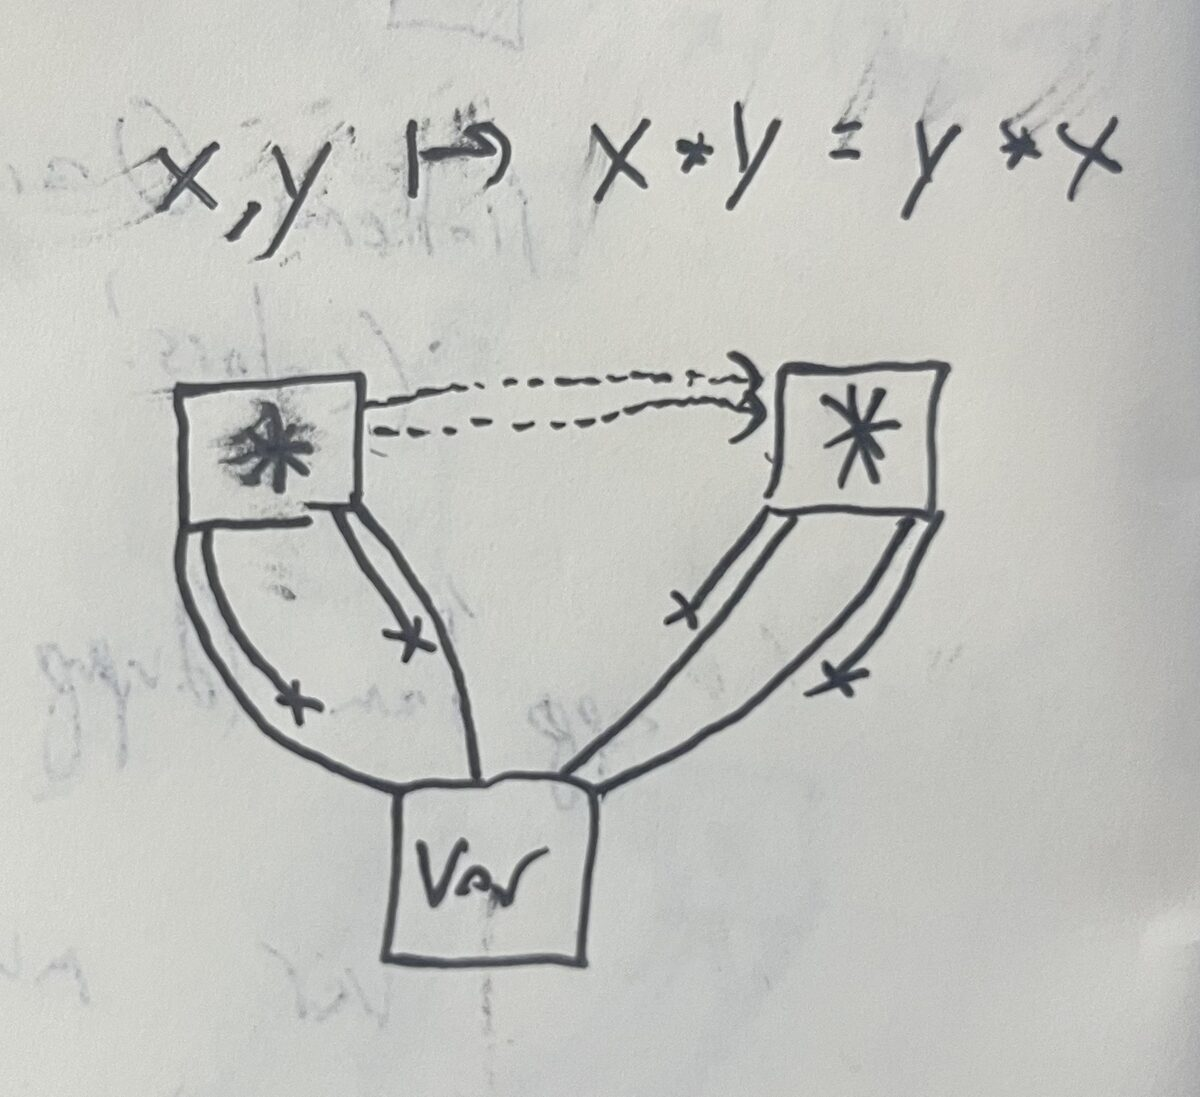
\includegraphics[width=0.5\linewidth]{thinegraphxyyx.jpg}
\caption{ A visualization of a lifting e-graph via thickening all edges into thinnings. This lifting e-graph represents $\text{lift}_{10}(\text{var}) * \text{lift}_{01}(\text{var}) \rightarrow \text{lift}_{01}(\text{var}) * \text{lift}_{10}(\text{var})$
}
\label{fig:liftegraph}
\end{figure}




\section{E-Matching}

E-matching in the typical case proceeds by composing thinnings as you traverse into rules. This is justified as an application of the lift pushing rule $\text{lift}_t(f(e_1, e_2)) \rightarrow f(\text{lift}_t(e_1),\text{lift}_t(e_2) )$

$$
\begin{aligned}
\mathrm{lift}_i(e_1)
  &=_? f(?a, ?b)
  && \text{goal} \\
\mathrm{lift}_i(f(e_2,e_3))
  &=_? f(?a, ?b)
  && \text{nondet e-class expand } e_1 \rightarrow f(e_2,e_3) \\
f(\mathrm{lift}_i(e_2), \mathrm{lift}_i(e_3))
  &=_? f(?a, ?b)
  && \text{lift-pushing}\\
\Rightarrow \quad
?a &= \mathrm{lift}_i(e_2) \quad \land \quad
?b = \mathrm{lift}_i(e_3)
  && \text{decompose } f
\end{aligned}
$$

There is more complexity coming from redundancies in union find $e_{\text{child}} \rightarrow \text{lift}_k(e_{\text{parent}})$.

The simplest choice of dealing with these is to have the match fail when it encounters these. E-matching into these expressions will be rewriting in expressions that are using variables in a redundant way. This is not likely to be a useful place to be spending computation.

However, if one does want to match into these, it is possible. It corresponds to solving for thinnings in the equation $\text{lift}_i(e_\text{parent}) = \text{lift}_{?j}(\text{lift}_k(e_\text{parent}))$, which may have multiple solutions. This corresponds in the named representation to $(x,y \mapsto 0) =_? (x,y \mapsto ?a * 0)$ having both $?a = x$ and $?a = y$ as solutions.

% All of the implementation of a lifting egraph was pretty mechanical without thinking too deeply until I hit e-matching. That is what sent me back to the drawing board to clarify the semantics and first order term model of what I was doing.

% A confusing thing is that we have made liftings baked in and somewhat implicit. Should liftings appear in patterns? When should liftings be allowed to be inserted to solve the problem?

% I think what I now understand is that there are at least 3 different e-matching problems you might want to solve.

% \begin{enumerate}
% \item $\texttt{0 = ?x * ?y}$ only matching on unlifted canonical id
% \item $\texttt{lift\_010(0) = ?x * ?y}$ matching a lifted id
% \item $\texttt{?lift1 0 = ?lift2 (?x * ?y)}$ matching an TBD arbitrarily lifted id.
% \end{enumerate}

%The last one is lightly a unification problem (has variables on both sides of the equations), so maybe we can consider that out of scope. It is a somewhat natural thing to ask though.

%By far the simplest thing to do, and I think it kind of makes pragmatic sense, is that as soon as you encounter a thinning from the root in the union find during ematching, just don't traverse that edge. This kind of corresponds to only solving problem 1. The only nodes you're going to find down that edge will contain redundant variables. It is rarely a good thing to have extra unnecessary variables around (they are expensive for all kinds of reasons), so why even do it? In this case, e-matching is basically identical to ordinary ematching but you do have to compose the thinnings as you are traversing down the argument edges of an enode.

%Ok, but let us say we want to do it.

%The pattern $\texttt{lift\_00(0) = ?x * ?y}$ with $x_{10} * \lift_0(0) = \lift_0(0)$ in the egraph should have 2 solutions, $\texttt{\{?x -> x20, ?y -> 0\}}$ and $\texttt{\{?x -> x21, ?y -> 0\}}$. This corresponds to matching against the target $x,y \mapsto 0$ and getting the two solutions $x,y \mapsto x * 0$ and $x,y \mapsto y * 0$. If we pattern match over an higher lifting of 0 like $\lift_{0000}(0)$, we'd expect 4 solutions, and so on. These are enumerating all the variables you can place in that spot that get annihilated by 0. In terms of the liftings, they are all the ways of solving the equation $\lift_{00} = \lift_? \cdot \lift_0$ which has two solutions $\lift_{10}$ and $\lift_{01}$. In words, to throw away both arguments $\lift_{00}$, you can either throw away the second argument and the one left $\lift_{10} \cdot \lift_0$, or you can throw away the first argument and then throw away the one left $\lift_{01} \cdot \lift_0$.

% $\lift_0 = \lift_? \cdot \lift_{00}$ problems of this shape have no solutions in liftings. Liftings monotonically increase the number of arguments, and $\lift_{00}$ has already lifted to taking in 2 redundant arguments whereas the left hand side  $\lift_0$ only takes in 1 redundant argument.

% Fully writing out the derivations of these two matches:

% \begin{lstlisting}
% lift_00(0) =? ?x * ?y
% lift_01(lift_0(0)) =? ?x * ?y               by lift factoring (motivated by the next move)
% lift_01(x10 * lift0(0)) =? ?x * ?y          by  lift_0(0) = x10 * lift0(0)
% lift_01(x10) * lift_01(lift0(0)) =? ?x * ?y by  mul-homomorphism   lift(mul(X,Y)) = mul(lift(X), lift(Y))
% ?x -> lift_01(x10), ?y -> lift_00(0)        by the usual syntactic matching of *
% \end{lstlisting}

% But you can also use the other factoring

% \begin{lstlisting}
% lift_00(0) =? ?x * ?y
% lift_10(lift_0(0)) =? ?x * ?y               by the other lift factoring (motivated by the next move)
% lift_10(x10 * lift0(0)) =? ?x * ?y          by  lift_0(0) = x10 * lift0(0)
% lift_10(x10) * lift_10(lift0(0)) =? ?x * ?y by  mul-homomorphism   lift(mul(X,Y)) = mul(lift(X), lift(Y))
% ?x -> lift_10(x10), ?y -> lift_00(0)        by the usual syntactic matching of *
% \end{lstlisting}


% \begin{figure}[htbp]
% \centering
% 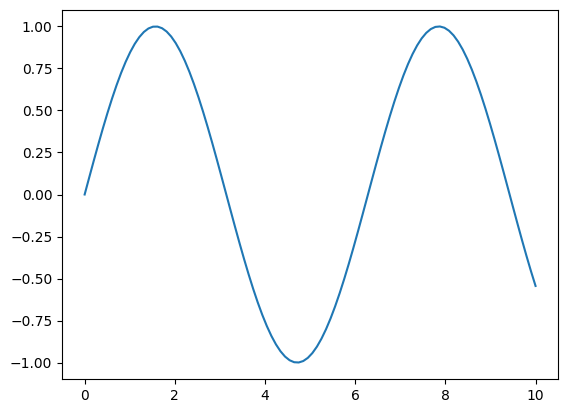
\includegraphics[width=0.5\linewidth]{2026-04-18-thin_egraph_files/2026-04-18-thin_egraph_2_1.png}
% \caption{$x \mapsto \sin(x) : R \to R$}
% \label{fig:sin-r-to-r-ematching}
% \end{figure}




% - Redundancies in union find $e_{\text{child}} \rightarrow \text{lift}_k(e_{\text{parent}})$ are trickier
%   - Choice 1: Don't Match Through Them
%   - Choice 2: Factor $\text{lift}_i(e_\text{parent}) = \text{lift}_{?j}(\text{lift}_k(e_\text{parent}))$
%     - Multiple solutions
%       - Ex: $(x,y \mapsto 0) =_? (x,y \mapsto ?a * 0)$
%       - solutions $?a = x$ and $?a = y$


\section{Related Work}

Slotted e-graphs \cite{slotted} are a mechanism for efficient handling of $\alpha$ equivalence in e-graphs. The e-graph described in this work can be seen as an approach to taking the slotted notion of redundancy as primary and removing the notion of permutative renaming. This is to some degree how the idea was developed. Both this work and slotted are related to the concept of Hashing modulo alpha equivalence \cite{hashalpha}, but it is not always clear how to take the ideas there and make them work in the highly shared situation of e-graphs.

Co de-Bruijn notation \cite{McBride_2018} is also a direct inspiration for the Thinning e-graph. Essentially the thinning e-graph is just an application of the Co de-Bruijn ideas in the e-graph setting.

The pointwise functional semantics is inspired by the semantics of judgements in type theory $\llbracket x : \mathbb{R}, y : \mathbb{R} \vdash \sin(x) : \mathbb{R} \rrbracket$. Indeed, the notation $\mapsto$ could be replaced throughout by $\vdash$, but this brings in new connotations. 

Weakening, Lifting, and Thinning are very similar concepts. There exists prior work on explicit Weakening calculi.

There are de Bruijn methodologies that allow the $succ$ constructor of the variables float inside of expressions rather than being tied to the variable \cite{kiselyov}\cite{pavel}. Every variable is associated with the $zero$ constructor then.

\section{Acknowledgements}
Many discussions with Rudi Schneider about slotted e-graphs have heavily informed this work. Commentary by Conor McBride on Mastodon about thinnings kicked off this particular branch of ideas. I'd also like to thank Max Willsey and Cody Roux for many interesting and relevant discussions.
\bibliographystyle{plain}
\bibliography{thinning}


\end{document}
